\documentclass[sigconf]{acmart}

%% CBSoft ACM-like adaptations
\settopmatter{printacmref=false}
\renewcommand\footnotetextcopyrightpermission[1]{}
\setcopyright{none}

\acmConference[SE4AS 2026]{1st Workshop on Software Engineering for
Agentic Systems}{September 8, 2026}{IME-USP, São Paulo, SP, Brazil}

\usepackage{enumitem}
\usepackage{tikz}
\usetikzlibrary{shapes.geometric, arrows.meta, positioning}

\AtBeginDocument{\providecommand\BibTeX{{Bib\TeX}}}

\begin{document}

%% TODO: título temporário — substituir por título focado no ângulo
%% multi-agente antes da submissão (exigência do SE4AS)
\title[GenAI and Software Engineering]{Generative Artificial
Intelligence and Software Engineering: Challenges and Opportunities}

\author{Gabriel Ferreira Silva}
\affiliation{
  \institution{Instituto de Informática, Universidade Federal de Goiás}
  \city{Goiânia}
  \country{Brazil}
}
\email{ferreira.silva@discente.ufg.br}

\author{Jacson Rodrigues Barbosa}
\affiliation{
  \institution{Instituto de Informática, Universidade Federal de Goiás}
  \city{Goiânia}
  \country{Brazil}
}
\email{jacson@inf.ufg.br}

\renewcommand{\shortauthors}{Silva and Barbosa}
\renewcommand{\shorttitle}{GenAI and Software Engineering}

\begin{abstract}
%% TODO: escrever após ter os números experimentais finais (WER, F1,
%% Cronbach, cobertura). Manter como parágrafo único sem quebras.
\end{abstract}

\keywords{Requirements Engineering, Multi-Agent Systems, Generative
AI, Speech-to-Text, User Stories, Agentic Systems}

\frenchspacing
\maketitle

%%=============================================================
\section{Introduction}
\label{sec:introduction}

Requirements engineering (RE) is a fundamental phase of software
development, bridging stakeholder needs and technical implementation.
In most organizations, requirements are gathered through meetings
facilitated by specialized professionals—requirements analysts,
product owners, or scrum masters—whose role is to accurately capture
complex, evolving discussions and transform them into formal artifacts
\cite{bokhari2011metrics}. This manual workflow introduces well-known
risks: information loss caused by memory decay between the meeting and
the documentation step, cognitive overload on the analyst who must
simultaneously participate and record, and inconsistency in granularity
and format across the resulting artifacts. Because requirements
documents serve as the foundation for every subsequent development
decision, poor or incomplete specifications translate directly into
misaligned implementations, rework, and cost overruns.

Commercial meeting intelligence tools—such as Fellow.ai
\cite{fellow2025}, Jamie \cite{jamie2025}, and Otter.ai—automate
transcription and action-item extraction but produce general-purpose
notes rather than formal software requirements artifacts. The
translation from meeting discussion to a structured Software
Requirements Specification (SRS) remains a manual, expertise-intensive
step. In the academic literature, studies applying Large Language
Models (LLMs) to RE address predominantly isolated subtasks: user
story generation from existing textual requirements
\cite{delgado2024aidriven}, conceptual model extraction
\cite{ren2024combining}, or requirements classification; few works
explore complete end-to-end pipelines from raw meeting audio to
stakeholder-specific, formally structured documentation
\cite{motger2025share}.

This work addresses the gap through a \emph{multi-agent architecture}
in which four specialized agents collaborate to transform meeting audio
into requirements documentation. Decomposing the pipeline into
agents—rather than a single monolithic LLM prompt—provides concrete
engineering advantages: (i)~\textit{separation of concerns}, enabling
each agent to be developed, tested, and evolved independently;
(ii)~\textit{entry-point flexibility}, allowing users to join the
pipeline at any stage (e.g., starting from an existing recording or
transcription); (iii)~\textit{per-agent model selection}, matching LLM
capability and cost to task complexity; and (iv)~\textit{observable
error propagation}, making it possible to trace and measure how
transcription errors cascade into downstream artifacts—a first-class
engineering concern in agentic systems.

Initial experiments with Agents~1 and~2—conducted as part of this
research—demonstrated 100\% persona identification accuracy (28/28
personas across 7 AMI meetings) and 83\% INVEST compliance in
generated user stories. This paper extends that implementation to its
\emph{complete form}, adding Agents~3 and~4 for requirements document
generation and domain diagram synthesis, introducing two selectable
output formats (IEEE~830 SRS and a client-specific format), and
conducting real-world validation on an actual government software
project. It also replaces the preliminary qualitative evaluation with
a quantitative harness covering transcription accuracy, information
extraction metrics, practitioner survey, and cross-pipeline error
propagation analysis.

\subsection{Research Questions}

This paper addresses the following research questions:

\begin{enumerate}[label=\textbf{RQ\arabic*.}]
  \item What is the automatic transcription accuracy (WER/CER) of
        Agent~1 for Portuguese meeting audio?
  \item How accurately does Agent~2 identify stakeholder personas and
        generate user stories (Precision/Recall/F1, INVEST compliance)?
  \item What is the perceived quality of the generated requirements
        document as evaluated by practitioners (structured survey)?
  \item How completely does the generated document cover a manually
        produced official requirements specification (P/R/F1)?
  \item How do errors propagate across pipeline stages, and how does
        per-agent model selection affect the cost--quality trade-off?
\end{enumerate}

\subsection{Main Contributions}

The main contributions of this work are:

\begin{enumerate}
  \item A complete, open-source 4-agent multi-agent system for
        end-to-end requirements elicitation from meeting audio,
        supporting two document formats (IEEE~830 SRS and a
        client-specific format).
  \item Real-world validation on a government software project, with a
        manually produced official requirements document as ground
        truth.
  \item A quantitative evaluation covering WER/CER (Agent~1),
        Precision/Recall/F1 with inter-rater agreement via Cohen's
        kappa (Agent~2), and a Likert-scale practitioner survey with
        Cronbach's alpha reliability assessment (Agent~3).
  \item A structured empirical analysis of cross-agent error
        propagation in an agentic pipeline, with per-stage latency and
        API cost measurements.
\end{enumerate}

The remainder of this paper is organized as follows.
Section~\ref{sec:related} reviews related work on LLMs in RE,
automated user story generation, and multi-agent systems.
Section~\ref{sec:method} presents the system architecture and the
real-world case study. Section~\ref{sec:evaluation} describes the
evaluation design. Section~\ref{sec:results} reports results and
discussion. Section~\ref{sec:threats} addresses threats to validity.
Section~\ref{sec:conclusion} concludes with future work.

%%=============================================================
\section{Related Work}
\label{sec:related}

\subsection{Large Language Models in Requirements Engineering}

The application of Large Language Models to requirements engineering
has attracted growing interest~\cite{hort2025survey}. Motger et
al.~\cite{motger2025share} conducted a systematic mapping study
identifying 62 publicly available datasets for LLM-based RE research,
finding that only 2 address elicitation tasks and that 58 of 62 are
English-only—a scarcity that directly motivates Portuguese-language
validation such as that presented here.

Regarding artifact generation, Delgado et
al.~\cite{delgado2024aidriven} compared N-gram heuristics with GPT-3
for automated user story generation from existing textual
specifications, reporting ROUGE-N\,=\,0.46 and BERTScore\,=\,0.69
for the LLM-based approach. Ren et al.~\cite{ren2024combining} further
showed that Chain-of-Thought prompting enables LLMs to extract
conceptual class diagrams from user stories. Naimi et
al.~\cite{naimi2024automating} leveraged LLMs to generate descriptive
use case text from UML diagrams encoded as XML, reducing documentation
time while improving consistency. Collectively, these works demonstrate
LLM viability for generating RE artifacts, but share a common
prerequisite: structured textual input. None addresses the extraction
of requirements from unstructured meeting audio.

\subsection{Speech Recognition for Meeting Transcription}

Automated speech recognition (ASR) is the enabling technology for
audio-based requirements elicitation. Radford et
al.~\cite{whisper2022} introduced Whisper, a large-scale weakly
supervised model demonstrating robust multilingual transcription across
diverse acoustic conditions, including non-native speakers and
background noise—characteristics common in real stakeholder meetings.
Kasakowskij and Haake~\cite{kasakowskij2025talk2text} developed
T$^3$~Talk2Text, a near-real-time ASR system for virtual group
meetings that captures full-group transcripts for downstream analysis
of communication and collaboration patterns.

Despite these advances, ASR in requirements elicitation meetings faces
domain-specific challenges: technical vocabulary, overlapping speech,
and project-specific acronyms that general-purpose models may
transcribe incorrectly. Such errors do not remain isolated—they
propagate to downstream agents, a failure mode we analyze empirically
as~RQ5.

\subsection{User Story Quality and the INVEST Framework}

User stories are the predominant requirements artifact in agile
development, following the format \textit{``As a role, I want goal so
that benefit''}~\cite{lucassen2016qus}. Wake~\cite{wake2003invest}
proposed the INVEST heuristics—Independent, Negotiable, Valuable,
Estimable, Small, Testable—as six criteria for assessing whether a
user story is actionable and well-scoped.

Lucassen et al.~\cite{lucassen2016qus} formalized the Quality User
Story (QUS) framework comprising 13 criteria covering syntax,
semantics, and pragmatics, and introduced AQUSA, an NLP-based tool
that detects quality defects. Evaluated on 1,023 stories from 18
software organizations, AQUSA demonstrates the feasibility of
automated quality assessment but requires manually written stories as
input. Xu et al.~\cite{xu2023requirement} combined INVEST with a
seven-criteria model to automate quality evaluation in agile
pipelines. Our work extends this thread by generating user stories
from meeting audio and evaluating them against INVEST using an
LLM-judge protocol validated against human raters.

\subsection{Multi-Agent Systems for Software Engineering}

Multi-agent architectures have emerged as a productive paradigm for
automating complex software engineering tasks. ChatDev~\cite{qian2024chatdev}
introduced a chat-powered framework in which specialized LLM agents
collaborate through structured dialogues across design, coding, and
testing phases, demonstrating that linguistic communication can
unify autonomous agents. MetaGPT~\cite{hong2024metagpt} encoded
Standardized Operating Procedures (SOPs) into prompt sequences,
assigning software engineering roles—product manager, architect,
engineer, QA—to distinct agents, achieving state-of-the-art results
on code generation benchmarks. Luo et al.~\cite{luo2024repoagent}
applied an agentic pipeline to documentation, with three specialized
agents producing and maintaining repository-level code documentation
that surpasses human-authored baselines. A recent survey by Cai et
al.~\cite{cai2025designing} analyzed 94 papers on LLM-based
multi-agent systems for SE tasks, finding that \textit{Role-Based
Cooperation} is the most commonly adopted design pattern—the same
pattern underlying our pipeline.

The closest work to ours is MARE~\cite{jin2024mare}, a multi-agent
collaboration framework for the entire RE process. MARE decomposes RE
into four tasks (elicitation, modeling, verification, specification)
across five specialized agents, outperforming state-of-the-art RE
baselines by up to 15.4\% in F1. However, MARE operates from a
textual \textit{rough idea} provided by a human and simulates
elicitation through agent-to-agent dialogue; it does not process
meeting audio and therefore cannot be deployed in a post-meeting,
fully automated scenario. Our system addresses precisely this gap.

\subsection{Identified Gaps}

The reviewed literature reveals four gaps that motivate this work:

\begin{enumerate}
  \item \textbf{Absence of audio-to-SRS pipelines.} Existing
        commercial tools~\cite{fellow2025,jamie2025} produce
        general-purpose meeting notes, not formal RE artifacts. LLM-based
        RE systems such as MARE~\cite{jin2024mare} process structured
        text, not raw conversational audio.

  \item \textbf{Isolated subtask focus.} Prior LLM work on RE addresses
        individual tasks—user story generation~\cite{delgado2024aidriven},
        use case description~\cite{naimi2024automating}, conceptual
        modeling~\cite{ren2024combining}—without integrating
        transcription, persona identification, and document generation
        into a single pipeline.

  \item \textbf{Lack of real-world validation.} Most studies use
        synthetic datasets or controlled corpora; few evaluate against a
        manually produced official requirements document from an actual
        software project.

  \item \textbf{Unanalyzed error propagation.} In agentic pipelines,
        transcription errors cascade into downstream artifacts. This
        failure mode is acknowledged but not empirically measured in any
        related work.
\end{enumerate}

This paper addresses all four gaps through a 4-agent pipeline that
transforms meeting audio into structured requirements documentation,
validated on a real government software project with quantitative
measurement of cross-agent error propagation.

%%=============================================================
\section{Method}
\label{sec:method}

\begin{figure}[tb]
\centering
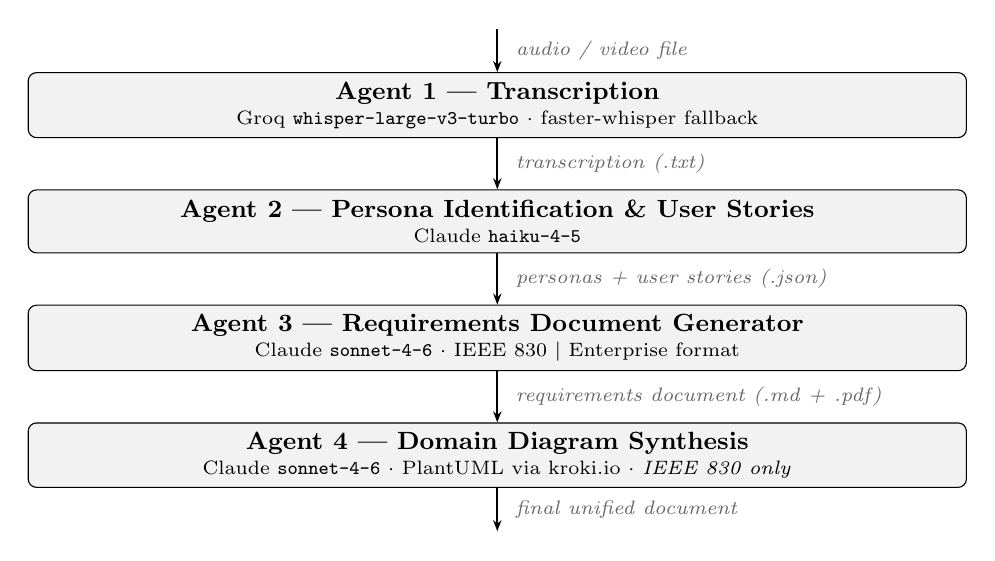
\begin{tikzpicture}[
  node distance=0.45cm,
  box/.style={draw, rounded corners=3pt, fill=gray!10,
              minimum width=\columnwidth-6pt, minimum height=0.80cm,
              align=center, font=\small\bfseries},
  art/.style={font=\scriptsize\itshape, text=black!60},
  arr/.style={-{Stealth[length=4pt]}, thick}
]
  \node[box] (a1)
    {Agent 1 --- Transcription\\[-2pt]
     {\normalfont\scriptsize Groq \texttt{whisper-large-v3-turbo}
       $\cdot$ faster-whisper fallback}};

  \node[box, below=0.65cm of a1] (a2)
    {Agent 2 --- Persona Identification \& User Stories\\[-2pt]
     {\normalfont\scriptsize Claude \texttt{haiku-4-5}}};

  \node[box, below=0.65cm of a2] (a3)
    {Agent 3 --- Requirements Document Generator\\[-2pt]
     {\normalfont\scriptsize Claude \texttt{sonnet-4-6}
       $\cdot$ IEEE~830 \textbar{} Enterprise format}};

  \node[box, below=0.65cm of a3] (a4)
    {Agent 4 --- Domain Diagram Synthesis\\[-2pt]
     {\normalfont\scriptsize Claude \texttt{sonnet-4-6}
       $\cdot$ PlantUML via kroki.io
       $\cdot$ \textit{IEEE~830 only}}};

  \draw[arr] ([yshift=0.55cm]a1.north)
    -- node[art,right=3pt]{audio / video file} (a1.north);

  \draw[arr] (a1.south)
    -- node[art,right=3pt]{transcription (.txt)} (a2.north);

  \draw[arr] (a2.south)
    -- node[art,right=3pt]{personas + user stories (.json)} (a3.north);

  \draw[arr] (a3.south)
    -- node[art,right=3pt]{requirements document (.md + .pdf)} (a4.north);

  \draw[arr] (a4.south)
    -- node[art,right=3pt]{final unified document} ([yshift=-0.55cm]a4.south);
\end{tikzpicture}
\caption{Four-agent pipeline. Agents communicate via a shared file
system monitored by watchdog. Agent~4 is skipped in enterprise-format
runs.}
\label{fig:architecture}
\Description{Five nodes connected vertically by arrows: an audio/video
input at the top, followed by four agents (Transcription, Identification,
SRS Generator, Diagram Synthesis) with intermediate file artifacts
labelled on each arrow, ending in a final document output at the
bottom.}
\end{figure}

\subsection{System Overview and Architecture}

The proposed system comprises four specialized agents connected
through a file-based sequential pipeline, as illustrated in
Figure~\ref{fig:architecture}. Each agent monitors the output
directory of its predecessor using the watchdog library; upon
detecting a new file, it triggers processing automatically without
manual intervention. This design provides loose coupling between
stages, fault isolation, and auditable intermediate artifacts. Users
may join the pipeline at any stage—supplying raw audio, an existing
transcription, or a prior analysis JSON—enabling partial reuse of
results across runs.

The pipeline supports two selectable output formats, chosen once per
run: \textbf{IEEE~830}, the standard Software Requirements
Specification structure used throughout this research; and
\textbf{Enterprise}, a client-specific document layout requested by
the industrial partner (Section~\ref{sec:casestudy}). In enterprise
runs, Agent~4 is skipped, as the client format does not include domain
diagrams. The format affects only the document template and some
agent prompts; all upstream stages (transcription, persona
identification, user story generation) are format-agnostic.

\subsection{Agent Design}
\label{sec:agents}

\subsubsection{Agent 1 --- Meeting Transcription}

Agent~1 accepts any audio or video file and produces a plain-text
transcription. Processing begins with \textbf{ffmpeg} normalization:
the input is converted to a 16~kHz mono FLAC file, reducing size
while preserving transcription-relevant signal. If the normalized
file exceeds the Groq API size limit, it is split at silence
boundaries into chunks, each transcribed independently and merged
into a single output.

Transcription is performed by \textbf{Groq} running
{\ttfamily whisper-large-\penalty0 v3-turbo}~\cite{whisper2022,groq2025}, chosen
for its combination of high multilingual accuracy and low latency
via hardware-accelerated inference. If the Groq API is unavailable,
the agent falls back automatically to \textbf{faster-whisper}
running the \texttt{small} model locally~\cite{ctranslate2}, trading
accuracy for offline availability.

\subsubsection{Agent 2 --- Persona Identification and User Story
Extraction}

Agent~2 reads the transcription and executes two sequential LLM
calls using \textbf{Claude \texttt{haiku-4-5}}~\cite{anthropic2025claude}.
The first call identifies distinct stakeholder personas present in the
conversation, extracting for each: name or identifier, role, defining
characteristics, and representative dialogue excerpts. The second
call generates persona-specific user stories following the INVEST
criteria~\cite{wake2003invest} in the format \textit{``As a [persona],
I want [goal] so that [benefit].''} Decomposing identification and
generation into two calls reduces context interference and improves
output structure. Results are saved as a typed JSON document that
serves as the contract between Agents~2 and~3.

\subsubsection{Agent 3 --- Requirements Document Generation}

Agent~3 reads the JSON produced by Agent~2 and generates a
requirements document using \textbf{Claude \texttt{sonnet-4-6}}
with \textbf{Jinja2} templates. In IEEE~830 mode, the output follows
the standard SRS structure (introduction, general description,
stakeholders, functional requirements, user stories table). In
enterprise mode, it follows the client layout (functional features,
detailed functional requirements with comments, business rules,
use cases, non-functional requirements). The document is rendered
to Markdown and then to PDF via \textbf{WeasyPrint}, using CSS
Paged Media for table of contents with automatic page numbers.

\subsubsection{Agent 4 --- Domain Diagram Synthesis}

Agent~4 is active only in IEEE~830 runs. It reads both the Agent~3
document and the original Agent~2 JSON, and uses \textbf{Claude
\texttt{sonnet-4-6}} to extract domain entities and their
relationships. The resulting PlantUML class diagram is rendered to
PNG via the \textbf{kroki.io} public API~\cite{groq2025} and embedded
in a final unified requirements document that consolidates all
previous sections.

\subsection{Model Selection Strategy}

Model selection per agent reflects an explicit cost--quality
trade-off. Agent~2 performs structured extraction with a well-defined
output schema (typed JSON); the task is repetitive and runs on every
meeting, making cost-per-call a primary concern---hence the use of
the lighter \texttt{haiku-4-5} model. Agents~3 and~4 perform
open-ended synthesis and document generation requiring stronger
reasoning and language fluency; \texttt{sonnet-4-6} is used for
both. Agent~1 uses a dedicated ASR model (Whisper) rather than a
general-purpose LLM, as speech recognition is a specialized task
for which Whisper achieves substantially better accuracy and speed.

\subsection{Real-World Case Study}
\label{sec:casestudy}

To validate the system in an authentic setting, we established a
partnership with the technology team of a Brazilian public sector
agency. The team provided a recorded stakeholder meeting and a
manually produced official requirements document for the same system,
which serves as ground truth for evaluation (RQ3--RQ4).

The meeting involved \textbf{10 participants} and ran for
\textbf{1~hour, 37~minutes, and 47~seconds}, conducted entirely in
Brazilian Portuguese. The subject was the redesign of a budget balance
management module in a government financial planning system. The raw
video file (609~MB) was processed end-to-end by the pipeline: ffmpeg
normalization, silence-based chunking, Groq transcription, persona
identification, and enterprise-format document generation.

The enterprise format was adopted at the partner's request, as the
organization does not use IEEE~830 internally. This requirement
motivated the dual-format architecture: the core data extraction
stages are format-agnostic, and the document format is a configurable
output parameter. The generated document and the official gold-standard
document are compared quantitatively in Section~\ref{sec:evaluation}.

%%=============================================================
\section{Evaluation Setup}
\label{sec:evaluation}

%% TODO

%%=============================================================
\section{Results and Discussion}
\label{sec:results}

%% TODO

%%=============================================================
\section{Threats to Validity}
\label{sec:threats}

%% TODO

%%=============================================================
\section{Conclusion and Future Work}
\label{sec:conclusion}

%% TODO

%%=============================================================
\section*{Artifact Availability}

The source code, evaluation scripts, and generated artifacts produced
in this research are publicly available at
\url{https://github.com/gabrielsfg/PFC1} under the MIT License.

\bibliographystyle{ACM-Reference-Format}
\bibliography{references}

\end{document}
